\documentclass[a4paper]{article}

% CUSTOM maketitle
\makeatletter
 \def\@maketitle{%
  \newpage
  \null
  \vskip 1.em
  \begin{center}%
  \let \footnote \thanks
    {\LARGE \bfseries\@title \par}%
    \vskip 1.em%
    {\large \langCourse \par}%
     {\large \langInstitute \par}%
    \vskip 1.em%
    {\large
      \lineskip .5em%
      \begin{tabular}[t]{c}%
        \@author { --- } \@istid \\
        {\href{mailto:\@email}{\tt\@email}}
      \end{tabular}\par}%
          \vskip 1.em%
    {\large \langAdvisor: \@advisor \par}%
    
  \end{center}%
  \par
  \vskip 1em}
\makeatother


% Commands to allow defining title, name, etc.
\makeatletter
\newcommand{\@StoreIn}[2]{ \gdef#1{#2} }
\newcommand*{\email}[1]{\@StoreIn{\@email}{#1}}
\newcommand*{\istid}[1]{\@StoreIn{\@istid}{#1\thanks{\langThanks}}}
\newcommand*{\advisors}[1]{\@StoreIn{\@advisor}{#1}}
\makeatother

% The 'utf8' package contains support for using UTF-8 as input encoding. 
\usepackage[utf8]{inputenc}
% The 'babel' package may correct some hyphenation issues of LaTeX. 
% Select your MAIN LANGUAGE for the Thesis with the 'main=' option.
\usepackage[english,portuguese]{babel}
\usepackage{iflang}
% Language dependent section names
\addto\captionsenglish{
  \renewcommand{\contentsname}{\null ~\vskip 1.em \hfil Contents\hfil}
  \renewcommand{\refname}{Bibliography}
}
\addto\captionsportuguese{
  \renewcommand{\contentsname}{\null ~\vskip 1.em \hfil Conteúdos\hfil}
  \renewcommand{\refname}{Bibliografia}
}

% Solves some font enconding issues related to the output
\usepackage[T1]{fontenc}

% These packages are typically required. 
% Among many other things they add the possibility to put symbols in bold
% by using \boldsymbol (not \mathbf); defines additional fonts and symbols;
% adds the \eqref command for citing equations.
\usepackage{mathtools, amsmath, amsthm, amssymb, amsfonts}
\usepackage{nicefrac}
%

% Tikz  for creating graphics programmatically.
\usepackage{tikz}
\usetikzlibrary{shapes.geometric, arrows, positioning}

% These packages are most usefull for advanced tables. 
% 'multirow' allows to join rows throuhg the command \multirow which works
% similarly with the command \multicolumn.
% The 'colortbl' package allows to color the table (foreground and background)
% The package 'booktabs' provide some additional commands to enhance
% the quality of tables
% The 'longtable' package is only required when tables extend beyond the length
% of one page, which typically does not happen and should be avoided
\usepackage{array}
\usepackage{booktabs}
\usepackage{multirow}
\usepackage{colortbl}
\usepackage{spreadtab}
\usepackage{longtable}
\usepackage{pdflscape}
\usepackage{float}

% Set links for references and citations in document
\usepackage{hyperref}
\hypersetup{ colorlinks=true,
             citecolor=cyan,
             linkcolor=darkgray,
             urlcolor=teal,
             breaklinks=true,
             bookmarksnumbered=true,
             bookmarksopen=true,
}

% Provides better support for handling and breaking URLs.
\usepackage{url} 

% The package 'graphicx' supports formats PNG and JPG.
% Package 'subfigure' allows to place figures within figures with own caption. 
% For each of the subfigures use the command \subfigure.
\usepackage{graphicx}
\usepackage[hang,small,bf,tight]{subfigure}

\usepackage[format=hang,labelfont=bf,font=small]{caption} 
% the following customization adds vertical space between caption and the table
%\captionsetup[table]{skip=10pt}

% These packages are required for list code snippets.
\usepackage{xcolor}
\usepackage{color}
% The following special color definitions are used in the IST Thesis
\definecolor{forestgreen}{RGB}{34,139,34}
\definecolor{orangered}{RGB}{239,134,64}
\definecolor{lightred}{rgb}{1,0.4,0.5}
\definecolor{orange}{rgb}{1,0.45,0.13}	
\definecolor{darkblue}{rgb}{0.0,0.0,0.6}
\definecolor{lightblue}{rgb}{0.1,0.57,0.7}
\definecolor{gray}{rgb}{0.4,0.4,0.4}
\definecolor{lightgray}{rgb}{0.95, 0.95, 0.95}
\definecolor{darkgray}{rgb}{0.4, 0.4, 0.4}
\definecolor{editorGray}{rgb}{0.95, 0.95, 0.95}
\definecolor{editorOcher}{rgb}{1, 0.5, 0} % #FF7F00 -> rgb(239, 169, 0)
\definecolor{chaptergrey}{rgb}{0.6,0.6,0.6}
\definecolor{editorGreen}{rgb}{0, 0.5, 0} % #007C00 -> rgb(0, 124, 0)
\definecolor{olive}{rgb}{0.17,0.59,0.20}
\definecolor{brown}{rgb}{0.69,0.31,0.31}
\definecolor{purple}{rgb}{0.38,0.18,0.81}

%For enhanced enumeration of lists
%\usepackage{enumitem}
\usepackage[shortlabels]{enumitem}
\setlist[description]{leftmargin=\parindent,labelindent=\parindent,itemsep=1pt,parsep=0pt,topsep=0pt}

% For rotating
\usepackage{rotating}
% For Gantt chart generation
\usepackage{pgfgantt}
% For dummy text generation
\usepackage{lipsum} 

% To define margins to be OF THE SAME DIMENSIONS AS DEI MASTER TEMPLATE
\usepackage{geometry}
\geometry{ 
  a4paper,         
  inner=1in,
  outer=1in,
  headheight=16pt,
  % textheight=637pt, 
  % textwidth=455pt,
  marginparsep=0pt,
  headsep=25pt,
  top=106pt,
  marginparwidth=56pt,
    heightrounded,   % integer number of lines
}

% The package 'acronym' garantees that all acronyms definitions are 
% given at the first usage. 
% IMPORTANT: do not use acronyms in titles/captions; otherwise the definition 
% will appear on the table of contents.
\usepackage[printonlyused]{acronym}

% BIBLIOGRAPHY related packages
\usepackage{cite}
\bibliographystyle{IEEEtran}
\usepackage{ulem}

% TITLE related packages  
\usepackage[runin]{abstract}

% To insert good looking code
\usepackage{listings}
\lstdefinestyle{mystyle}{
    backgroundcolor=\color{white},   % choose the background color
    basicstyle=\ttfamily\small,      % the size of the fonts used for the code
    breakatwhitespace=false,         % sets if automatic breaks should only happen at whitespace
    breaklines=true,                 % sets automatic line breaking
    captionpos=b,                    % sets the caption-position to bottom
    commentstyle=\color{green!40!black},  % comment style
    keywordstyle=\color{blue},       % keyword style
    keywordstyle={[2]\color{purple!80!black}}, % additional keywords
    keywordstyle={[3]\color{orange}}, % additional keywords
    identifierstyle=\color{black},   % identifier style
    numberstyle=\tiny\color{gray},   % the style used for line-numbers
    numbers=left,                    % where to put the line-numbers
    numbersep=5pt,                   % how far the line-numbers are from the code
    stringstyle=\color{orange},      % string literal style
    showspaces=false,                % show spaces everywhere adding particular underscores
    showstringspaces=false,          % underline spaces within strings only
    showtabs=false,                  % show tabs within strings adding particular underscores
    tabsize=4,                       % default tabsize
    emph={int,char,double,float,unsigned,void},
    emphstyle={\color{blue}},
    emph={[2]for, while, do, if, else, switch, case},
    emphstyle={[2]\color{purple!80!black}},
    emph={[3]printf, scanf, cout, cin, endl, include},
    emphstyle={[3]\color{orange}}
}
% Use the defined style for code listings
\lstset{style=mystyle}

% Set language dependent texts
\newcommand{\keywords}[1]{\IfLanguageName{english}{\\[10pt]\textbf{{Keywords ---}} #1}{\\[10pt]\textbf{{Palavras Chave ---}} #1}}
\newcommand{\langAdvisor}{\IfLanguageName{english}{Advisor(s)}{Orientador(es)}}
\newcommand{\langCourse}{\IfLanguageName{english}{PIC2 - Master in Computer Science and Engineering}{PIC2 - Mestrado em Engenharia Informática e de Computadores}}
\newcommand{\langInstitute}{\IfLanguageName{english}{Instituto Superior Técnico, Universidade de Lisboa}{Instituto Superior Técnico, Universidade de Lisboa}}
\newcommand{\langThanks}{\IfLanguageName{english}{I declare that this document is an original work of my own authorship and that it fulfills all the requirements of the Code of Conduct and Good Practices of the Universidade de Lisboa (\url{https://nape.tecnico.ulisboa.pt/en/apoio-ao-estudante/documentos-importantes/regulamentos-da-universidade-de-lisboa/}).}{Declaro que o presente documento é um trabalho original da minha autoria e que cumpre todos os requisitos do Código de Conduta e Boas Práticas da Universidade de Lisboa (\url{https://nape.tecnico.ulisboa.pt/en/apoio-ao-estudante/documentos-importantes/regulamentos-da-universidade-de-lisboa/}).}}


% acmart uses Libertine for text, Inconsolata for monospaced font and newtxmath for math:
\usepackage[varqu]{zi4} 
\usepackage{newtxmath}


\begin{document}

%%%%%%%%%%%%%%%%
% TITLE & NAME %
%%%%%%%%%%%%%%%%
% \selectlanguage{portuguese}  % <-- ACTION: UNCOMMENT for english or portuguese
\selectlanguage{english}  % <-- ACTION: UNCOMMENT for english or portuguese
\title{A Process Framework for Human–AI Collaboration in the Software Development Lifecycle} % <-- ACTION: WRITE your project title here
% A Process Framework for AI adoption in the Software Development Lifecycle
\author{Tomás dos Santos Taborda} % <-- ACTION: WRITE your complete name here
\istid{103641} % <-- ACTION: WRITE your student number  here (your student number, not the IST-ID)
\email{tomassantostaborda@tecnico.ulisboa.pt} % <-- ACTION: WRITE your e-mail here
\advisors{Miguel Mira da Silva, Hugo de Sousa} % <-- ACTION: WRITE your advisor name here

% To make the title
\maketitle
\thispagestyle{empty}

%%%%%%%%%%%%
% ABSTRACT %
%%%%%%%%%%%%
% To remove indentation before abstract
\setlength{\abstitleskip}{-\absparindent}
\begin{abstract}
The rise of Generative Artificial Intelligence (GenAI) and Large Language Models (LLMs) is transforming software engineering by enabling natural-language-driven development and accelerating tasks across the Software Development Life Cycle (SDLC). While these technologies introduce new possibilities for automation, productivity, and early-stage support for the software development workflow, they also raise concerns regarding reliability, security, transparency, and long-term maintainability. A Systematic Literature Review (SLR) done about the use and adoption of AI in Software Development reveals a major problem: despite rapid adoption, organizations lack structured methodologies to integrate AI and LLMs into development workflows in a responsible, value-driven, and accountable manner. This absence of guidance forms the core research problem.

To address this problem within the Software Development environment, the report proposes a new framework inspired by Agile and Scrum principles to support the adoption, collaboration, and governance of AI-assisted development practices. The framework aims to define phases, practices, and oversight mechanisms for integrating AI throughout the SDLC. Its applicability will be explored through a demonstration within a next-generation consultancy, followed by an evaluation involving practitioners, experts, and analytical criteria. Together, these steps establish the foundation for a structured, evidence-based approach to Human–AI collaboration in software engineering.
\keywords{Vibe Coding, AI, Gen AI, LLM, Software Engineering, Software Development, Software Development Lifecycle, Scrum, Agile,  AI Adoption, Human-AI Collaboration, Benefits, Consequences, Methodologies, Framework} % <--- ACTION: WRITE YOUR KEYWORDS HERE
\clearpage
\end{abstract}

%%%%%%%%%%%%%%%%%%%%%
% TABLE OF CONTENTS %
%%%%%%%%%%%%%%%%%%%%%
\tableofcontents
\thispagestyle{empty}
\clearpage


%% <-- ACTION: ADD/EDIT/REMOVE/COMMENT SECTIONS IF YOU NEED TO
%%%%%%%%%%%%%%%%
% INTRODUCTION %
%%%%%%%%%%%%%%%%

\section{Introduction}

The software engineering landscape is currently undergoing a significant change due to the rapid evolution of Artificial Intelligence. Specifically, the rise of Generative AI and Large Language Models has extended beyond simple classification tasks to enable the generation of coherent, context-aware outputs, reshaping traditional problem-solving and creative workflows across the technology sector.

Within this context, these technologies are revolutionizing the Software Development Life Cycle (SDLC) by introducing "Vibe Coding" and intent-driven programming, where developers collaborate with models using natural language. This paradigm shift automates complex tasks from code generation to documentation, but also necessitates a transition from manual code construction to a role focused on oversight, validation, and architectural decision-making to maintain high standards of reliability, security and quality.

To investigate the Software Development environment landscape rigorously, this report employs a dual methodological approach comprising a Systematic Literature Review (SLR) and the Design Science Research Methodology (DSRM). The SLR, following Kitchenham’s guidelines, was conducted to map the current state of AI adoption, benefits, and consequences, while the DSRM provides the structured process for designing, developing, and validating the proposed solution artifact.

Despite the rapid adoption of these tools, the industry faces a critical problem, and therefore it is defined a research problem: the absence of established, solid, and clear methodologies to guide the responsible integration of AI and LLMs into professional workflows. Existing research remains fragmented across isolated tools, leaving organizations without a structured approach to manage the risks regarding trust, explainability, and long-term maintainability that accompany AI-assisted development.

Addressing this gap, this report proposes a new framework inspired by Agile and Scrum principles designed to support the adoption, collaboration, and governance of AI-assisted development practices. This artifact defines specific phases, practices, and oversight mechanisms to integrate AI throughout the SDLC, ensuring that the technology enhances productivity without compromising value or accountability.

The applicability of this framework is demonstrated through a realistic project scenario within a next-generation consultancy. This demonstration illustrates how the proposed artifact functions in a real-world setting, guiding a team through the challenges of Vibe Coding and AI-augmented prototyping while maintaining alignment with business goals.

To validate the proposal, an ex post evaluation strategy is outlined, involving interviews with practitioners and Agile experts alongside an analytical assessment against defined success criteria. This evaluation aims to confirm the framework's utility, feasibility, and alignment with industry needs, ensuring it effectively supports Human-AI collaboration.

The remainder of this report is structured to guide the reader through the research process: Section 2 details the methodologies used; Section 3 provides the theoretical background; Section 4 presents the findings of the Systematic Literature Review; Section 5 defines the research problem; Section 6 outlines the objectives; Section 7 introduces the proposed framework; and Sections 8 through 11 cover the demonstration, evaluation plan, communication strategy, and final conclusions.





%%%%%%%%%%%%%%%%%%%%%%%
% Research Metodology %
%%%%%%%%%%%%%%%%%%%%%%%
\input{Sections/ResearchMetodology}

%%%%%%%%%%%%%%%%%%%%%%%
% Research Background %
%%%%%%%%%%%%%%%%%%%%%%%
\input{Sections/ResearchBackground}

%%%%%%%%%%%%%%%%%%%%%%%
% Systematic Literature Review %
%%%%%%%%%%%%%%%%%%%%%%%
\input{Sections/SystematicLiteratureReview}

%%%%%%%%%%%%%%%%%%%%%%%
% Research Problem %
%%%%%%%%%%%%%%%%%%%%%%%
\section{Research Problem}

This section presents the first step of the Design Science Research Methodology (DSRM), the identification of the problem, and its motivation. 

As shown in the results in Tables 5, 6, 7, 8 and 9 to the research questions, a lot of sectors can take advantage of the AI and LLMs transformative assets, incorporate it into their workflow. Although AI has been in the Software Development landscape for a while now, due to the highly dynamic and fast-evolving nature of the field, new models and new tools are being created nearly every month, and AI usage in general has never been so prevalent not only in the Software Development field but in other industry sectors as well. 

The conclusions drawn from the information collected in the systematic literature review, indicate that while many benefits can be attained from the use of AI, many challenges and disadvantages are in the way of its successful implementation and usage. Therefore the real main challenge organizations face and one of the most important consequences that is mentioned within the literature is the lack of established, solid and clear methodologies, that shape the proper use of AI and LLMs within the Software Development realm and across the industry and professional practice. \cite{Banh:2025cf, Farhanna:2025eu, Hemmat:2025rd, Gao:2025cc}

Although several frameworks and approaches that incorporate AI into the development process have been proposed, as summarized in Table 7, these solutions differ significantly in scope, assumptions, and level of abstraction. They often lack a shared foundation regarding lifecycle integration, management practices, and evaluation criteria. Consequently, organizations face difficulties not only in adopting AI-supported development practices, but also in objectively assessing their impact on software quality, security, and maintainability due to the lack of standardized benchmarks and performance metrics; ultimately proving that the field is actively searching for structured and repeatable integration patterns and methodologies. \cite{Ahmed:2025ai}

This problem is further amplified by the fact that AI increasingly influences all phases of the SDLC. Due to this problem, companies are seeking for a new methodological evolution to fully embrace, utilize, incorporate and implement AI and LLMs into their workflow. Traditional methodologies such as Waterfall, Scrum, Kanban, and the Agile Manifesto introduced substantial improvements in adaptability and collaboration, but they were not designed for development environments in which AI or LLMs actively contribute to software creation. \cite{Zhang:2025ea}

As a result and as AI-assisted development becomes more prevalent, modern development teams experience new dynamics, including the rise of Vibe Coding, accelerated implementation, emerging bottlenecks created by AI in earlier phases such as requirements clarification and later phases such as testing, and a stronger emphasis on delivering product value rather than merely increasing feature output. Together, these changes indicate that existing methodologies may no longer fully align with emerging AI-augmented development dynamics. Existing traditional frameworks often fall short in AI-driven contexts because:

\begin{itemize}
    \item high-speed AI-assisted coding accelerates implementation but creates pressure upstream (requirements clarification) and downstream (testing, verification, and maintenance);
    \item they lack explicit structures for AI governance, prompt engineering, model reliability assessment, and risk mitigation;
    \item they assume all contributors are humans, whereas AI models introduce a new category of collaborator.
\end{itemize}

\textbf{Therefore, the core research problem addressed in this work is the lack of patterned guidance, strict methodologies and standardized evaluation metrics that can be defined through a structured, process-oriented framework that supports the systematic integration and management of AI and LLM-based tools across the Software Development Lifecycle, while preserving human oversight, software quality and security, and organizational accountability. This gap limits organizations’ ability to fully and sustainably realize the potential benefits of AI-assisted software development.}



%%%%%%%%%%%%%%%%%%%%%%%
% Research Objective %
%%%%%%%%%%%%%%%%%%%%%%%
\section{Research Objective}

This section aims to clarify the objective of this research.

From the conducted systematic literature review, it was possible to gather an overview of the current status of the topic of AI and LLMs usage adoption in regards to Software Development. With the analysis of the consequences and benefits that these tools have, a research problem was defined in the previous section, namely, the lack of patterned guidance, strict methodologies and standardized evaluation metrics to fully make the most of out of the potential that AI and LLMs can bring to an information rich environment. Therefore, the research objectives of this work are defined to directly address the research problem identified in the previous section. This problem, grounded in the findings of the Systematic Literature Review, concerns the lack of structured guidance, methodological rigor, and standardized evaluation practices for integrating AI and LLMs into software development processes. Table 13 summarizes how the research objectives are formulated to resolve this problem, linking the identified gaps to concrete framework objectives.

{\small
\begin{longtable}{>{\raggedright\arraybackslash}p{0.6cm} 
                  >{\arraybackslash}p{5.3cm} 
                  >{\arraybackslash}p{3.2cm} 
                  >{\arraybackslash}p{5.2cm}}
\caption{Mapping between Research Questions, Key Findings, Problem Aspects, and Framework Objectives}
\label{tab:rq_objective_mapping} \\

% Header for the first page
\toprule
\textbf{RQ} & \textbf{Key Finding from SLR} & \textbf{Problem Aspect Addressed} & \textbf{Resulting Framework Objective} \\
\midrule
\endfirsthead

% Header for continuation pages
\toprule
\textbf{RQ} & \textbf{Key Finding from SLR} & \textbf{Problem Aspect Addressed} & \textbf{Resulting Framework Objective} \\
\midrule
\endhead

\midrule
\multicolumn{4}{r}{\textit{Continued on next page}}\\
\endfoot

\bottomrule
\endlastfoot

RQ1 &
The analysis of benefits and usage patterns shows that AI and LLM usage is unevenly distributed across SDLC phases and lacks structured integration. &
Lack of structured guidance on where and how AI should be applied across the SDLC &
Define a process framework that explicitly maps AI-supported activities to specific SDLC phases, clarifying where and how AI tools should be applied. \\
\addlinespace

RQ2 &
The analysis of consequences and limitations highlights recurring risks related to reliability, validation, security, and insufficient human oversight. &
Insufficient methodological support for managing risks, quality, and accountability in AI-assisted development &
Integrate governance mechanisms, human-in-the-loop practices, and quality assurance checkpoints into the framework. \\
\addlinespace

RQ3 &
The review of existing methodologies reveals significant variation among approaches and a lack of consensus on how to manage AI adoption in software development. &
Fragmentation and lack of consensus in existing AI adoption methodologies &
Consolidate best practices into a unified, process-oriented framework that provides repeatable guidance for managing human–AI collaboration. \\
\addlinespace

\end{longtable}
}


Together, these objectives operationalize a solution to the identified research problem by translating observed gaps in current practice into concrete design goals for the proposed framework. By explicitly mapping AI usage to SDLC phases, introducing governance and human-in-the-loop mechanisms, and consolidating fragmented practices into a unified process model, the framework aims to resolve the lack of structured guidance and methodological clarity currently limiting the effective and responsible adoption of AI and LLMs in software development.


%%%%%%%%%%%%%%%%%%%%%%%
% Research Proposal %
%%%%%%%%%%%%%%%%%%%%%%%
\section{Research Proposal}

This section delineates the proposal to address the research problem identified in Section 5. 

This research proposes the development of a process-oriented framework to support the adoption, structural integration, and ongoing management of AI and LLM-based tools within Software Development processes. The proposal is motivated by the lack of structured and standardized guidance identified in the systematic literature review, particularly regarding how organizations can responsibly incorporate these technologies while preserving software quality and security, development integrity, and human oversight.

The proposed framework views AI and LLM-based tools as collaborative development services operating alongside human developers throughout the Software Development Lifecycle. Rather than positioning AI as an autonomous code generator, it emphasizes human–AI co-development, where AI systems provide computational and generative support while human professionals remain responsible for correctness, security, compliance, architectural soundness, and alignment with business requirements. Unlike traditional Agile and Scrum-based methodologies, which assume exclusively human contributors, the framework explicitly treats AI systems as first-class socio-technical actors whose contributions, limitations, and risks must be managed throughout the SDLC.

To operationalize this perspective, the framework defines a structured set of phases, practices, evaluation metrics, and decision-making guidelines governing the lifecycle of AI integration in Software Engineering:

\begin{enumerate}
    \item \textbf{Adoption \& Strategy Definition}, assessing justification, feasibility, and intended AI roles;
    \item \textbf{Design \& Integration}, establishing practices for human–AI collaboration, prompt formulation, model selection, and environment adaptation;
    \item \textbf{Operation \& Quality Assurance}, ensuring reliability, security, and transparency through human-in-the-loop mechanisms;
    \item \textbf{Continuous Monitoring \& Improvement}, applying metrics and governance to detect risks such as vulnerabilities, bias, or declining code diversity.
\end{enumerate}

Organizations increasingly seek methodological evolutions beyond traditional Agile and Scrum frameworks to address environments where AI actively contributes to software creation. The proposed framework represents such an evolution. While inspired by their iterative and value-driven principles, it is designed to replace human-only development methodologies in contexts where AI systems actively contribute to software creation, redefining process structure, responsibilities, and governance to explicitly account for human–AI collaboration. In practical terms, the framework aims to support AI-driven prototyping without sacrificing requirement accuracy, integrate AI responsibly into development and testing activities, redefine collaboration roles, reduce risks such as hallucinations and unverified code, and enable development processes in which human judgment and AI capabilities reinforce one another.

Thus, the proposal of this research is to define, structure, and validate a process-oriented framework that formalizes AI as a collaborative actor, introduces lifecycle governance mechanisms, and supports accountable human–AI collaboration in software development, providing actionable guidance for organizations seeking to adopt AI tools in a secure, responsible, sustainable and value-driven manner. This involves not only describing the framework but demonstrating it in practice and evaluating its suitability for real development contexts.


%%%%%%%%%%%%%%%%%%%%%%%
% Demonstration %
%%%%%%%%%%%%%%%%%%%%%%%
\section{Demonstration}
In this section, the demonstration phase of the DSRM methodology is discussed. It illustrates how the proposed framework can be applied to address the research problem identified in Section 5 within a realistic software development context.

The research proposal includes the development of a process-oriented framework inspired by Agile and Scrum principles, aimed at providing actionable guidance for organizations seeking to adopt AI and LLM-based tools in a secure, responsible, sustainable, and value-driven manner. To demonstrate how the framework can be used in practice, a realistic project scenario is considered based on an next-generation consultancy.

This consultancy is a next-generation consultancy that helps organizations solve business problems with technology rapidly, creatively, and always with people at the centre. Unlike traditional consultancies or software houses, this consultancy prioritizes business value, high-speed delivery, and new ways of building, including Vibe Coding and AI-assisted prototyping. Their mission is to unlock progress where other approaches stall.

In the demonstration scenario, a team is tasked with developing a small to medium-sized software application. The organization already pioneers the use of AI, LLMs, and other AI-augmented tools to accelerate software development through practices such as Vibe Coding. The team operates using Scrum-based practices, short feedback cycles, and continuous alignment with stakeholders. However, despite this advanced adoption, this consultancy, like many modern consultancies, continues to seek new methodological evolutions of Scrum and Agile that can systematically standardize and govern the use of AI across the entire Software Development Lifecycle. In the absence of clear guidance and structured processes for integrating AI into development workflows, the team encounters challenges that are typical of AI related environments:
\begin{enumerate}
    \item difficulty validating and reviewing AI-generated code in a consistent and structured manner;
    \item increased pressure on requirements refinement, as rapid prototyping exposes ambiguities earlier in the process;
    \item increased complexity in functional and security testing due to unpredictable AI behaviour;
    \item unclear responsibility boundaries between human contributors and AI-generated artifacts.
\end{enumerate}

These challenges reflect the gaps identified in the systematic literature review and motivate the application of the proposed framework. Within this scenario, the framework is applied as the primary process structure to guide the adoption and integration of AI tools, define explicit human–AI collaboration practices, introduce human-in-the-loop quality assurance checkpoints, and guide decision-making across SDLC phases. Development artifacts such as AI-generated outputs, prompt formulations, review notes, and iteration-level observations are used to illustrate how the framework governs AI participation and supports accountable development practices.

The demonstration will be structured around a limited number of short development iterations aligned with Agile cycles. Across these iterations, the application of the framework focuses on observing decision points related to AI tool selection, prompt formulation, validation practices, and responsibility allocation between human developers and AI systems. The demonstration emphasizes process behavior rather than delivery performance, enabling the analysis of how the framework shapes development practices, oversight mechanisms, and collaboration patterns.

The next section focuses on evaluating the framework’s suitability, usefulness, and alignment with the needs observed in this scenario, in accordance with the Evaluation stage of the DSRM methodology.


%%%%%%%%%%%%%%%%%%%%%%%
% Evaluation %
%%%%%%%%%%%%%%%%%%%%%%%
\section{Evaluation}

This section details how the research proposal will be evaluated, which encompasses the evaluation stage of the DSMR methodology. Piers-Heje et al. differentiates two aspects of the evaluation of an IS artifact: when evaluation takes place and how it is evaluated, meaning the timing and environment of the evaluation. 

Given that the framework described in the research proposal section will be evaluated after it has been constructed and given that the evaluation of the proposed framework will be based on its actual use within a real development scenario, the evaluation will be “ex post” as opposed to “ex ante”, which would evaluate the design of the model before it was constructed and after its design. Since the evaluation will be carried out within an organization in a real-life scenario with real users, and as such in regards to the way the evaluation is conducted, it will be naturalist, in opposition to the artificial environment according to Piers-Heje et al \cite{J.Pries-Heje:2008SD}. The artifact will then be subjected to four types of evaluations, as shown in Figure 6:

\begin{itemize}
    \item \textbf{Demonstration:} The application of the proposed framework in a realistic organizational scenario will provide initial evidence of its usefulness, clarity, and effectiveness in guiding Human--AI collaboration in the context of an organization.
    \item \textbf{Practitioner Interviews:} Interviews with software developers, engineering managers, and AI practitioners will be conducted to collect insights regarding the practicality, feasibility, and perceived value of the framework in real development workflows.
    \item \textbf{Scrum/Agile Expert Interviews:} Agile coaches, Scrum masters, and product development experts will be consulted to evaluate how well the framework aligns with Agile principles, complements existing delivery methodologies, and addresses the emerging challenges of AI-augmented development.
   \item \textbf{Analytical Evaluation using Benchmarks and Success Criteria:} 
    The framework will be evaluated against predefined criteria, including clarity, completeness, alignment with SDLC phases, support for Human-in-the-Loop practices, and governance of AI-enabled activities. Each criterion will be assessed qualitatively using a three-level ordinal scale (low, medium, high), which is commonly used in qualitative DSR evaluations to indicate degree of satisfaction rather than precise performance measurement. Therefore indicating the extent, to which the framework satisfies each criterion, based on evidence gathered from the demonstration and expert feedback, with brief qualitative justifications grounded in observed usage, artifacts, and interview data.
\end{itemize}

\begin{figure}[H]
    \centering
    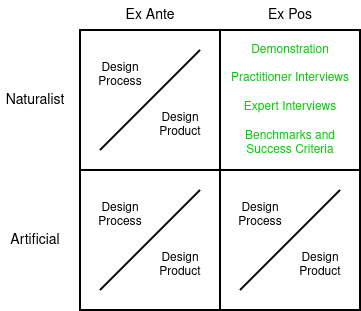
\includegraphics[width=0.33\linewidth]{Images/evaluation.png}
    \caption{Chosen approach for artifact evaluation (adapted from \cite{J.Pries-Heje:2008SD})}
    \label{fig:placeholder}
\end{figure}

The evaluation is expected to provide evidence regarding the practical suitability and perceived value of the proposed framework. It is anticipated that practitioners will highlight strengths such as improved guidance for Human-AI collaboration, clearer role definition, and enhanced structure for integrating AI tools across SDLC activities. Agile experts are expected to comment on how the framework aligns with or extends Agile principles, particularly in environments adopting Vibe Coding or AI-assisted development. However, certain limitations are acknowledged. As the evaluation is conducted within a limited number of organizational settings, broader generalization may be constrained. The scope of real-world application may also be limited by time, availability, or the maturity of AI tools in use. Finally, because the evaluation focuses on early practical adoption, long-term impacts such as organizational change or sustained performance improvements cannot yet be measured.

Despite these limitations, the evaluation is expected to provide a strong foundation for validating the relevance and applicability of the proposed framework and for identifying directions for future refinement and potential large-scale deployment.

%%%%%%%%%%%%%%%%%%%%%%%
% Communication %
%%%%%%%%%%%%%%%%%%%%%%%
\section{Communication}
This section reflects the communication step of the DSRM, which is the last step of this methodology. 

The plan includes the preparation of two scientific publications. The first publication will present the findings of the Systematic Literature Review on the adoption and use of AI and LLMs in Software Development. The second, which is this report, will focus on the proposed framework for managing Human–AI collaboration within organizational software engineering practices while also discussing the SLR findings. Only the first SLR scientific publication will be submitted to the ACM Transactions on Software Engineering and Methodology journal, while the second will be presented andd submitted to an academic examination committee.

Alongside these publications, a comprehensive final dissertation report will be produced, formally presented, defended, and evaluated by an academic examination committee.

%%%%%%%%%%%%%%%%%%%%%%%
% Conclusion %
%%%%%%%%%%%%%%%%%%%%%%%
\section{Conclusion}

This report started to investigate the transformative integration of Artificial Intelligence and Large Language Models into software engineering through a Systematic Literature Review that mapped current benefits, consequences, and stakeholder opinions. From the information collected in the SLR, it could be shown that while AI adoption is accelerating across the industry, organizations currently lack structured methodologies to integrate these tools responsibly without compromising software quality, security, or accountability. To address this gap, this research is proposing a new framework based on Agile and Scrum principles, designed to formalize Human-AI collaboration and guide the governance of AI-enabled development workflows.

The primary limitations of this study relate to the scope of its evaluation strategy. As the framework is assessed through a demonstration within a specific consultancy context and relies on qualitative expert interviews, the generalization of results to broader organizational settings may be constrained. Additionally, because the evaluation focuses on the initial stages of adoption, long-term impacts such as sustained organizational change and lasting performance improvements cannot yet be fully measured.

Future work will focus on the comprehensive development and refinement of the proposed framework, followed by its practical demonstration and "ex post" evaluation within the next-generation consultancy environment. This process will assess the artifact’s validity, practical suitability, and perceived value through the outlined interviews and success criteria. The research will culminate in the final dissertation and the submission of scientific papers, aiming to provide actionable standards for the responsible era of AI-augmented software development.



%%%%%%%%%%%%%%%%%%%%%%%
% Declaration of Use %
%%%%%%%%%%%%%%%%%%%%%%%
\section*{Declaration of use}

In the making of this report, several artificial intelligence tools were used to support the execution of specific tasks. ChatGPT and Gemini were used to assist with the overall structuring of the report, to support the summarization and condensation of section contents, to suggest alternative wording and synonyms, and to help organize selected phrases in order to improve clarity, coherence, and reduce redundancy. Rayyan was used to assist in the screening and selection of relevant studies based on predefined inclusion and exclusion criteria, as well as to facilitate duplicate removal and conflict resolution during the systematic literature review process. Google NotebookLM was used to support the collection and organization of information from the source literature for the purpose of answering the defined research questions.

All intellectual decisions, including article selection, the formulation of research questions, and the interpretation of findings, were made exclusively by the author. The AI tools were employed solely for support and did not produce any original content.

\textit{This Declaration of Use is in accordance with the guidelines of Instituto Superior Técnico.}


%%%%%%%%%%%%%%%%
% BIBLIOGRAPHY %
%%%%%%%%%%%%%%%%
% add Bibliography to TOC
\addcontentsline{toc}{section}{\refname}
% The following command resets the 'emphasis' style for bibliography entries
\normalem

% CHOOSE AND ADD YOUR STYLE HERE
\bibliographystyle{plain} % Or ieeetr, unsrt, apalike, etc.

% Name of your BiBTeX file
\bibliography{./Bibliography} % Make sure your file is named "Bibliography.bib"

% The following command modifies the 'emphasis' style for bibliography entries
\ULforem

%%%%%%%%%%%%%
%    END    %
%%%%%%%%%%%%%

\end{document}
